\documentclass[oneside,noframe]{ncuthesisXe}
\usepackage{makeidx}             % for index
\usepackage{layout}              % to show page dimensions
\usepackage[]{todonotes}         % Use [disable] to del. all
\usepackage{cite}
% 以下為中大碩博士論文封面輸入資料
\dept      {XXX研究所} 	%系所
\degree    {碩/博士}			%碩\博士
\title     {中文論文名稱}		%論文名稱
\subtitle  {English Thesis Title}		%論文名稱 英文
%\logo{NCUlogo}   %中央無校徽在封面,要除去校徽則用此行
\author    {作者}
\mprof     {指導教授}

\sprofi   {共同指導教授} 		%沒有共同指導教授請註解
\sprofii   {共同指導教授2}		%或把參數省略成為\sprofii{}	
\degreedate{中~華~民~國~一百零五~年~六~月}
\copyyear  {2016-2017}
\def\scalefactor{1}        % define a new command
\newcommand\insertfig[3]{
\renewcommand\scalefactor{#3}
\begin{figure}[!hbt]
\centering
\includegraphics[scale=\scalefactor]{#1}
\caption{#2}
\label{Fig:#1}
\end{figure}
}
\newtheorem{thm}{定理}[chapter]
\newtheorem{pr} {作業}[chapter]
\newtheorem{pf} {證明}[chapter]
\newtheorem{algo}{演算法}[chapter]

% what follows are for watermark, mark these out if no need
%\usepackage{background} 
%\SetBgContents{
\includegraphics{NCUlogo}} % need a watermark
%\SetBgAngle{0}                                           % rotate
%\SetBgColor{black!40}                                 % color
%\SetBgScale{1.5}                                          % scale
%\SetBgHshift{100}                                        % location x=0 for center
%\SetBgVshift{230}                                        % location y=0 for center
% end of watermark codes
               % 自訂巨集多 收起來,
                                 % 自訂巨集少 直接寫出

%\includeonly{introduction}          % 單獨編譯此檔
%\makeindex                       % 告訴\LaTeX要做索引
\begin{document}                 % 宣告結束,本文開始
%----------------------
\fontsize{14pt}{20pt}\selectfont % 可調間距以便閱讀

\maketitle                       % 論文封面							
\setboolean{printcopyright}{true}									
\maketitle                       % 書名面							
\addtocontents{toc}{~\hfill\textbf{頁次}\par}
\cleardoublepage 
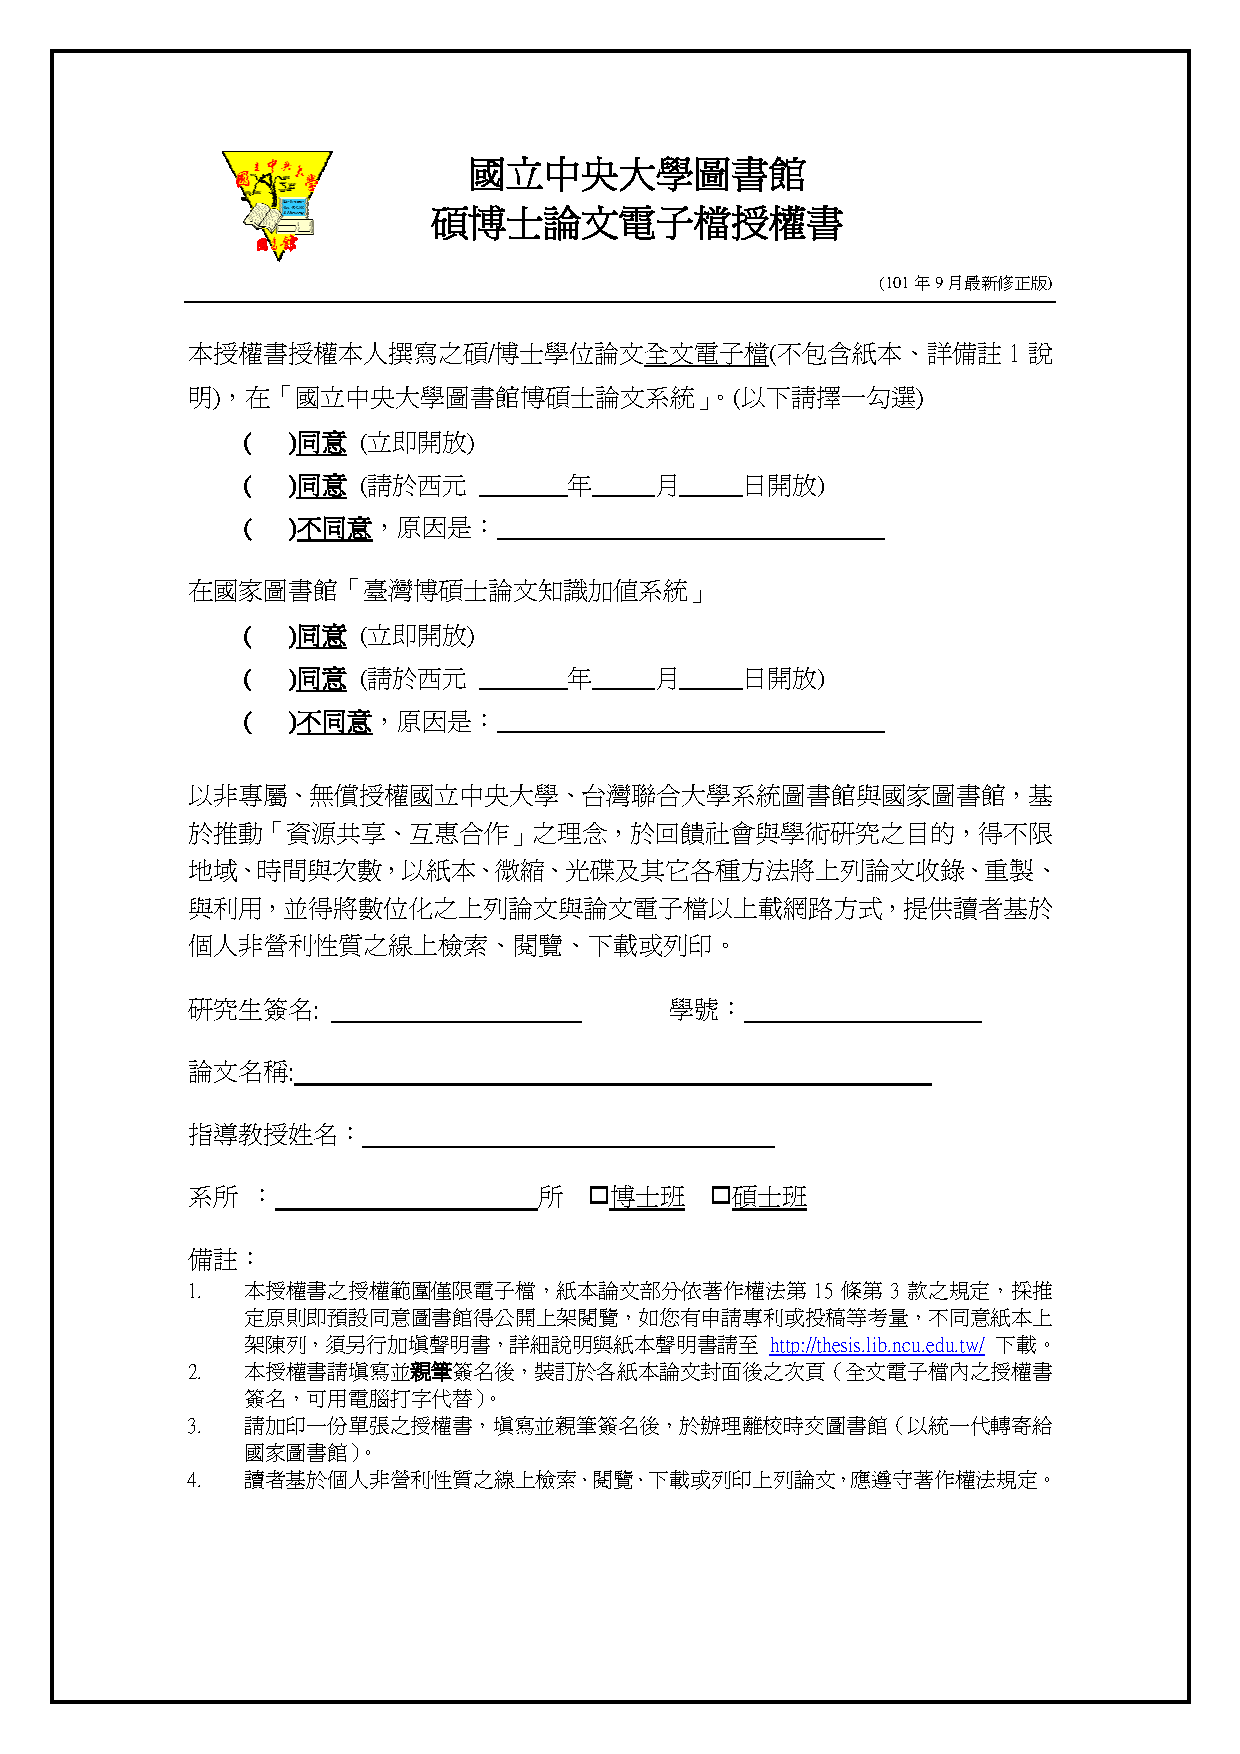
\includepdf[pages=-,scale=0.9]{myfile.pdf} % 插入其他表格  		

\frontmatter                     % 羅馬數字編頁
\begin{abstractcn}
\index{ncuthesis環境!abstractcn}
abstractcn
\end{abstractcn}              % 中文摘要abstractcn環境 			
\begin{abstracten}
\index{ncuthesis 環境!abstracten}
abstracten  sad
\end{abstracten}              % 英文摘要abstracten				
\begin{acknowledgements} \index{謝誌}
\index{ncuthesis 環境!acknowledgements}

\end{acknowledgements}             % 謝誌     acknowledge			
\cleardoublepage
\phantomsection\addcontentsline{toc}{chapter}{目錄}
\tableofcontents                 % toc
\cleardoublepage
\phantomsection\addcontentsline{toc}{chapter}{圖目錄}
\renewcommand{\numberline}[1]{圖~#1\hspace*{1em}}%圖目錄
\listoffigures                   % lof
\cleardoublepage
\renewcommand{\numberline}[1]{表~#1\hspace*{1em}}%表目錄
\phantomsection\addcontentsline{toc}{chapter}{表目錄}
\listoftables                    % lot
\index{\LaTeX!\textbackslash phantomsection}
\index{\LaTeX!\textbackslash addcontentline}
\index{\LaTeX!\textbackslash hspace}

\listoftodos
\todo[inline]{完稿時要用[disable]除去所有todos。}                  % 目錄  toc, lof, and lot
\begin{symbols}
\index{ncuthesis 環境!symbols}
\label{symb}
\end{symbols}                 % 符號說明   symbols 環境			

\cleardoublepage \index{\LaTeX! \textbackslash include}
\mainmatter                      % 阿拉伯數字編頁         
\chapter{緒論}
			 % 第一章    (自行寫入)
\chapter{相關研究}
\chapter{研究方法}

\chapter{結論}
~\nocite{*}						%show all you bib refernce paper,完成論文時請註解掉

\cleardoublepage                         % 保證奇數頁為章節起始
\phantomsection
\addcontentsline{toc}{chapter}{索引}     % 將索引加入目錄中

\printindex

\cleardoublepage                         % 保證奇數頁為章節起始
\phantomsection
\addcontentsline{toc}{chapter}{參考文獻}     % 將參考文獻加入目錄中

%\bibliographystyle{unsrt}      	
\bibliographystyle{IEEEbib}
\bibliography{myfoo}                   %參考文獻bib檔案 % 或標準資料庫用法





          
%\begin{thebibliography}{20}          % 文獻少寫法
%\bibitem{knu84}
%Donald E. Knuth. \emph{{The TEXbook, Volume A of Computers and Typesetting}}. \hskip 1em plus 0.5em minus
% 0.4em\relax Addison-Wesley, Reading, Massachusetts, second edition, 1984, ISBN 0-201-13448-9.\\
%\url{http://www-cs-staff.stanford.edu/~knuth/index.html}
%
%\bibitem{lam94}
%Leslie Lamport. \emph{{\LaTeX{}: A Document Preparation System}}. \hskip 1em plus 0.5em minus 0.4em\relax Addison-Wesley, Reading, Massachusetts, second edition, 1994, ISBN 0-201-52983-1.
%
%\bibitem{lo12a}
%J.~LO, \emph{{eThinking in Circuits with PSpice}}.\hskip 1em plus
% 0.5em minus 0.4em\relax Cavesbooks, Inc., 2012, \\ ISBN 978-957-41-8721-8.
%
%\bibitem{lo12b}
%------, \emph{{aThinking in Control with Matlab}}.\hskip 1em plus
%0.5em minus 0.4em\relax Cavesbooks, Inc., 2012, \\ ISBN pending.
%
%\bibitem{lo12c}
%------, \emph{\LaTeX\ \& U 自助出版}.\hskip 1em plus
%0.5em minus 0.4em\relax 中央敦煌, 北科文具部, 2012, \\ ISBN 978-957-41-9448-3.
%
%\bibitem{lo12d}
%------, \emph{Packages author of ncuthesis(CJK, Xe), bizcard, cnwritingCJK}.\hskip 1em plus
%0.5em minus 0.4em\relax Free packages, 2012.\\
%\url{https://code.google.com/p/ncu-thesis-latex-template/}
%\bibitem{}
%\emph{{Writing a thesis in \LaTeX}}
%\url{http://texblog.org/}
%
%\bibitem{126570}
%Chinese character \textbackslash cjk within \textbackslash section\{\} does not work using pdflatex, + \textbackslash includegraphics, \hskip 1em plus
%0.5em minus 0.4em\relax\\
%\url{http://tex.stackexchange.com/a/126570}
%
%\bibitem{79776}
%\emph{Page numbers only appear on pages where a chapter starts}, \hskip 1em plus
%0.5em minus 0.4em\relax\\
%\url{http://tex.stackexchange.com/a/79776}
%\end{thebibliography}                      % 少文獻寫法




%{\centering \layout}             % 整頁尺寸(可註解%不用)

\end{document}                   % 52 lines in total